% !TeX root = ../../tesis.tex
% §2.1.3 — movido de 3-1-4-Eficiencia.tex l. 11-112 (sin l. 33-40) y de
% 3-1-5-Interconectividad.tex l. 11-66 + fig. l. 97-107 (#36); Mishra unificado,
% cierre con Kujala nuevo. Se quedan en §3.1: 3-1-4 l. 113-121 y 3-1-5 l. 68-115.

% -----------------------------------------------------------------------
\subsection{Indicadores de Eficiencia, Accesibilidad e Integración}
\label{subsec:ea-indicadores}
% -----------------------------------------------------------------------

La eficiencia de una red de transporte se entiende, en su dimensión topológica,
como la capacidad del sistema para conectar cualquier par de puntos
origen-destino a través del camino de menor costo posible ---medido en términos
de tiempo de viaje, número de transbordos o distancia recorrida---. Esta
propiedad es directamente computable sobre el grafo de la red mediante
algoritmos de caminos mínimos, lo que la convierte en una de las métricas más
operativas del análisis propuesto en este trabajo.

\citet{fortin2016innovative} plantean que los indicadores derivados de la teoría
de grafos ---como el \termino{índice alfa} (grado de ciclicidad), el
\termino{índice gamma} (grado de conectividad) y el
\termino{índice de superposición de líneas}--- caracterizan la eficiencia del
diseño de la red de manera directamente relacionada con su topología. Sin
embargo, estos autores reconocen que tales indicadores no consideran las
características únicas del transporte público, como la frecuencia de servicio,
la posibilidad de transferencias entre líneas o la variabilidad del servicio a
lo largo del día; por ello proponen complementarlos con indicadores dinámicos
derivados del modelo de grafo expandido en el tiempo construido con datos
\gtfs{}. En este modelo, la eficiencia se mide a través del camino mínimo
ponderado en la dimensión temporal, que incorpora tiempos de espera y
frecuencias reales de cada línea.

La distribución de los flujos de tráfico a lo largo de la red determina, en gran
medida, su eficiencia operativa. Un sistema topológicamente bien diseñado puede
resultar ineficiente en la práctica si los flujos de demanda se concentran
desproporcionadamente sobre un subconjunto reducido de nodos o aristas,
generando congestión y tiempos de viaje superiores a los predichos por el modelo
teórico.

\citet{batista2015} proponen abordar este problema mediante una variación
ponderada de la \termino{centralidad de intermediación} (
\textit{betweenness centrality}), en la que el grafo de la red vial es ponderado
no solo por la longitud de las aristas, sino por el número de rutas generadas
por la demanda real de tráfico, representada mediante una matriz origen-destino
(\textsc{od}). En su marco teórico, un nodo o arista de alta centralidad de
intermediación es aquel que aparece con mayor frecuencia en los caminos mínimos
entre los pares origen-destino del sistema; los nodos con esta propiedad
concentran los flujos de manera natural y son, por tanto, los primeros en
colapsar ante un incremento de demanda o una perturbación. La eficiencia urbana
aumenta cuando el sistema logra redistribuir estos flujos hacia rutas
alternativas, reduciendo la dependencia de los nodos centrales y homogeneizando
la carga sobre la red.

Esta perspectiva es fundamental para el análisis de la red metropolitana objeto
del presente estudio: la identificación computacional de los arcos y nodos con
mayor centralidad de intermediación ponderada por la demanda permite señalar
aquellos segmentos del sistema donde las inversiones en infraestructura o las
modificaciones de rutas producirían las mayores ganancias en eficiencia global.

La eficiencia urbana no se agota en la optimización interna de los flujos de la
red; incluye también la dimensión espacial de la \termino{accesibilidad}, es
decir, la capacidad del sistema de transporte para garantizar que cualquier
usuario, independientemente de su ubicación en el territorio, pueda alcanzar una
cantidad mínima de destinos dentro de umbrales de tiempo razonables.

\citet{fortin2016innovative} señalan que los indicadores de accesibilidad más
comunes se calculan definiendo un radio de cobertura (por ejemplo, 500 metros
como distancia caminable aceptable) alrededor de las paradas de la red, y
evaluando la proporción de población o de empleos que quedan dentro de dicha
cobertura. Sin embargo, estos autores reconocen que este enfoque estático no
incorpora la demanda real de los usuarios ---representada por sus pares
origen-destino específicos--- ni la frecuencia del servicio, lo que limita su
capacidad para reflejar la experiencia real de accesibilidad. Proponen por ello
indicadores dinámicos que, construidos sobre el grafo ponderado en el tiempo,
permiten calcular la accesibilidad real desde cualquier nodo de la red hacia
todos los demás, considerando los horarios y frecuencias del servicio. Esta
\termino{accesibilidad dinámica}, calculada algorítmicamente sobre el modelo de
grafo, constituye una medida integral de la eficiencia urbana que se incorporará
al análisis computacional de la presente investigación. La
Figura~\ref{fig:indices-grafos} resume tres índices clásicos de teoría de
grafos que \citet{fortin2016innovative} retoman como antecedente, con sus
ventajas y sus limitaciones.

\begin{figure}[H]
   \centering
   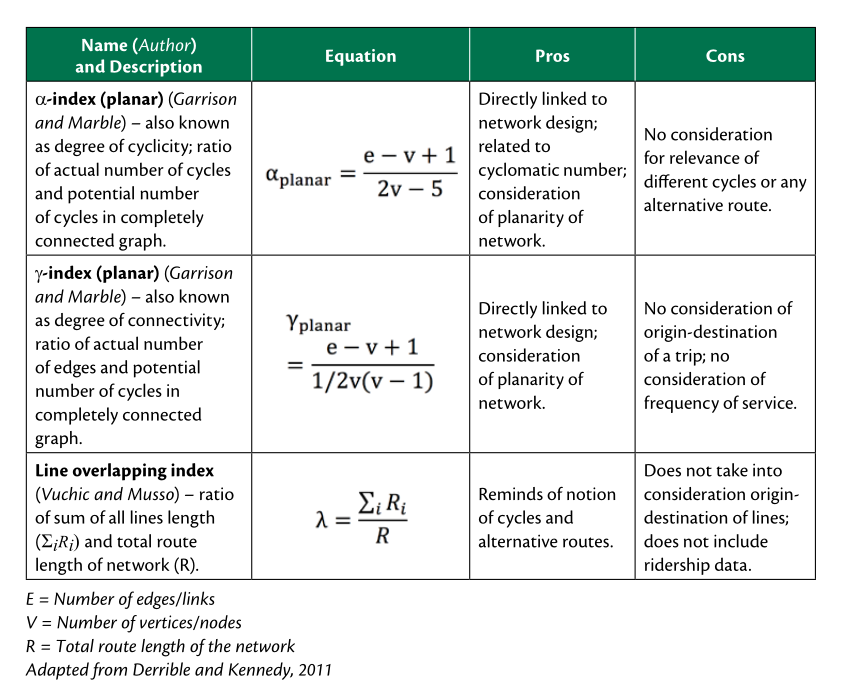
\includegraphics[width=0.85\textwidth]{Figures/Cap3/TablaIndicatorsAdaptedGraphTeory.png}
   \caption[Índices de Grafos \gtfs{}]{Tabla de indicadores de grafos \gtfs{}.
   Traducción: \textit{Name (Author) and Description}, nombre (autor) y
   descripción; \textit{Equation}, ecuación; \textit{Pros}, ventajas;
   \textit{Cons}, desventajas. Los índices son el $\alpha$ planar o grado de
   ciclicidad y el $\gamma$ planar o grado de conectividad, ambos de Garrison y
   Marble, y el índice de superposición de líneas, de Vuchic y Musso; $e$ es el
   número de aristas, $v$ el de vértices y $R$ la longitud total de las rutas.
   Tabla adaptada de Derrible y Kennedy (2011).}
   \label{fig:indices-grafos}
   \fuentefigura{\citet{fortin2016innovative}, p.~23.}
\end{figure}

Además de la eficiencia y la accesibilidad, la literatura mide la integración
entre modos. Se habla de interconectividad entre redes cuando metro, autobús,
trolebús, \brt{} y otros modos funcionan como un solo sistema, con transbordos
cortos y una cobertura que ninguno alcanzaría por su cuenta. En el grafo, esa
integración se dibuja con \termino{aristas de transferencia} entre nodos de
modos o líneas distintos; su peso incluye el tiempo de caminar entre andenes, la
espera y, si existe, una segunda tarifa.

\citet{ugur2025} afirman que la integración juega un papel crucial para
garantizar que los diferentes modos de transporte público operen de manera
armoniosa, facilitando las transferencias y permitiendo a los pasajeros
desplazarse con facilidad entre destinos. En un sistema bien integrado, la
fortaleza de la conexión entre líneas no solo amplía el área accesible para el
usuario, sino que también reduce las dificultades experimentadas durante el
viaje, lo que influye positivamente en la demanda de transporte público y
contribuye a la sustitución del vehículo privado. Su investigación sobre la
línea M7 del metro de Estambul demuestra que la evaluación sistemática de la
conectividad en cada estación ---mediante un
\termino{Índice de Conectividad Simplificado} (\textsc{sci}, por sus siglas en
inglés) que incorpora variables de velocidad, capacidad de pasajeros,
frecuencia, horas de operación y distancia al origen--- revela patrones de
integración desigual que orientan directamente las decisiones de inversión y
mejora operativa. La Figura~\ref{fig:sci-estambul} muestra el trazo de esa
línea y sus 17 estaciones.

\begin{figure}[H]
  \centering
  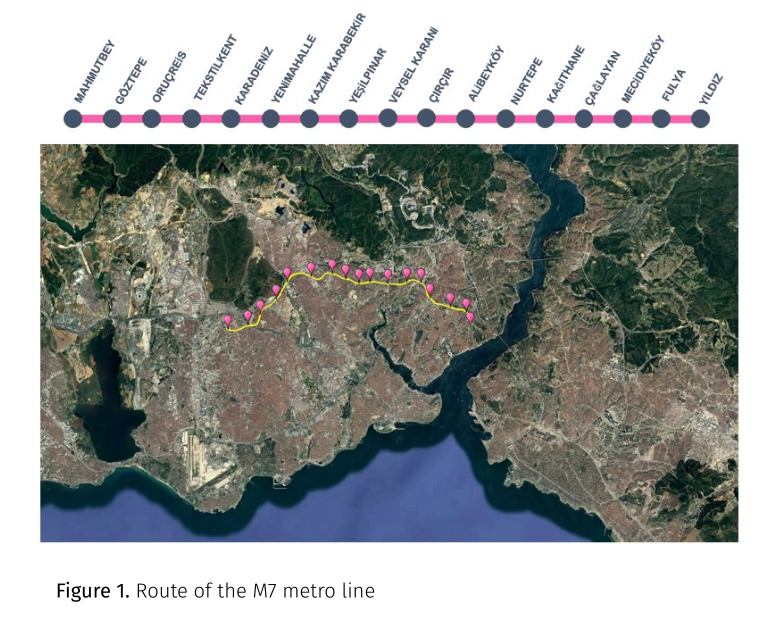
\includegraphics[width=0.88\textwidth]{Figures/Cap3/M7Estambul.png}
  \caption[Línea M7 del metro de Estambul]{%
  Trazo de la línea M7 del metro de Estambul y sus 17 estaciones, sobre la que
  \citet{ugur2025} calculan el \textsc{sci}. Traducción del rótulo:
  \textit{Route of the M7 metro line}, trazo de la línea M7 del metro;
  «Figure~1» es la numeración de la fuente.}
  \label{fig:sci-estambul}
  \fuentefigura{\citet{ugur2025}.}
\end{figure}

Para medir la interconectividad no basta contar cuántas líneas pasan por un
nodo; hay que medir qué tan buena es la conexión. \citet{mishra2015} evalúan la
conectividad en tres niveles: la parada, la línea y el centro de transferencia
(\termino{transfer center}). El índice de un nodo se obtiene de la suma de las
potencias de conexión de las líneas que pasan por él, y la potencia de cada
línea depende de su velocidad, distancia, frecuencia, tiempo de encabezamiento
(\termino{headway}), capacidad, aceleración y desaceleración, además de la
dirección de la ruta. Con esto, la eficiencia topológica y la operativa quedan
en una sola métrica por nodo, que esta tesis toma como referencia para construir
sus indicadores.

Este enfoque supera las limitaciones de la centralidad de grado simple, que
únicamente cuenta el número de conexiones directas de un nodo sin considerar la
calidad ni la frecuencia del servicio ofrecido. \citet{mishra2015} subrayan que
medir la conectividad puede resultar una tarea compleja y esquiva, pues es
necesario considerar tarifas, horarios, capacidad, frecuencia y otras
características del sistema en su conjunto; por ello, la evaluación de la
conectividad del transporte requiere un enfoque sistemático que integre los
múltiples parámetros involucrados en la prestación del servicio real. La
diferencia entre un sistema integrado y uno fragmentado se traduce directamente
en la magnitud de la \termino{penalización por transbordo} percibida por el
usuario: cuando la conectividad en los nodos de transferencia es alta, esta
penalización se reduce, haciendo el sistema más atractivo respecto al
automóvil.

Estos trabajos miden dimensiones distintas de la red: \citet{fortin2016innovative}
la eficiencia y la accesibilidad con los horarios reales del servicio,
\citet{batista2015} la concentración de los flujos en pocos nodos, y
\citet{mishra2015} y \citet{ugur2025} la calidad de la conexión en cada parada.
Cuando se quiere ver varias de esas dimensiones a la vez, la salida no es
obvia. \citet{kujala2018} normalizaron los datos \gtfs{} de 25 ciudades y
presentaron sus indicadores como un perfil por ciudad, sin reducirlos a un
índice global. Esa decisión es la que retoma la Clasificación Garibelt
(§\ref{subsubsec:garibelt-normalizacion}).
